\documentclass[11pt,letterpaper]{article}
\usepackage[utf8]{inputenc}
\usepackage{babel}
\usepackage{amsmath,
            amsfonts,
            amssymb}
\usepackage{graphicx}
\usepackage{minted}
\usepackage{float}
\usepackage{hyperref}

\title{\textbf{Solidspy\_DYN}: A Python based finite element code for dynamic analysis of elastic solids using implicit time integration}
\date{}
\author{Juan Gomez and Nicolas Guarin}

\usepackage{cleveref}
\begin{document}
\maketitle

\abstract{This tutorial describes the basic steps required in the construction of a finite element model using the Python based code {\bf Solidspy\_DYN}. The code has been written mainly for teaching purposes and also as a first hand calculator for complex wave propagation problems. {\bf Solidspy\_DYN} is written using Python but also makes extensive use of free open code software as {\bf gmsh} and {\bf Paraview} which are used for pre and post processing. This document describes  the steps involve in the creation of a {\bf gmsh} model to be used within the implicit time integrator. This is achieve through  a sample problem that is geometrically simple yet it involves all the basic parts that conform a {\bf Solidspy\_DYN} analysis. It is assumed that the user is familiar with general {\bf gmsh} syntaxis and features. The user manual is focused in the aspects required to complete a dynamic analysis thus emphasizing the visualization of the solution in the free code {\bf Paraview}.}

\section{Introduction}
The finite element method (FEM) or its variations, is probably the numerical technique of major use in modern engineering to the extent that it is included in a large number of engineering curriculum at the undergraduate and graduate level. Unfortunately many of these courses use as simulation tool specialized and expensive commercial software that, although powerful from a computational point of view is highly limited when used for teaching purposes as these codes are usually a black-box hiding most of its numerical methods to the student.The python based open code {\bf SolidsPy} has been written to be used mainly as a teaching tool since it is structured in such a way that its independent subroutines can be used to show the student the different steps in the  construction of a finite element algorithm. Furthermore, the code is open and can be modified to satisfy the needs of a learning process without any risk as it can be restored to its original version.

This document describes the steps required for the generation of a finite element model for elastic two-dimensional media to be analyzed with {\bf Solidspy\_DYN}. It walks the student/user through the complete modeling process starting with the definition of the domain using external free open software, continuing with the writing of input files for the code and finishing with solution visualization with additional external free open software.

The first part of the document describes how to define input data files to {\bf Solidspy\_DYN} in terms of simple text files. The next section shows the construction of complex geometric domains using {\bf gmsh}, the external and free mesh generation program. Then the manual describes the process of writing the input files using yet another external software corresponding in this case to the python based module {\bf meshio}. The final part of the document describes the postprocessing or visualization with {\bf Paraview}. 


In order to show the modeling process we use a simple problem and its {\bf gmsh} definition in terms of geometrical and physical entities as required to conduct dynamic analysis with {\bf Solidspy\_DYN}. The model to be analyzed is geometrically simple but it involves all the parts and steps required for the analysis. One of the main purposes in a dynamic analysis of continuum media is to capture the time history of the response of a given quantity. By default {\bf Solidspy\_DYN} writes the response time history in terms of displacements at every time step. The solution is written in the form of {\bf vtk} files ready to b visualized with {\bf Paraview}. This tutorial assumes that the user is familiar with the fundamental aspects of {\bf gmsh} and thus it is more focused in the parts required in the model so it can be analyzed with {\bf Solidspy\_DYN}.

To be able to follow this tutorial the user requires the following software:

\begin{itemize}
\item {\bf Solidspy\_DYN}: The dynamic version of the finite element analysis code {\bf Solidspy}.
\item {\bf Solidspy}: This basic code is required since we will used some of the libraries available in {\bf Solidspy}.
\item {\bf Gmsh}: The free mesh creation software.
\item {\bf meshio}: The input-output module to read and write the {\bf Gmsh} models.
\item {\bf paraview}: The free solutions visualization software. 
\end{itemize}

\section{Creating a model in SolidsPy\_DYN }
In general, a finite element model for the solution of the theory of elasticity boundary value problem (BVP) involves (i) a discretization or partition of the problem domain into sub-domains, also known as the mesh, (ii) a description of the boundary conditions and (iii) a description of the material properties. Dynamic problems also require the definition of time parameters like initial conditions and a description o the time behavior of loads.

A finite element mesh is nothing else than a discrete set of points (or nodes) arranged into so-called finite elements or subdomains. The method itself, is based upon the local solution of the BVP in each element within which the displacement field at an arbitrary point is expressed in terms of the displacements at the nodal points. Once the displacement field is known it can be used in the determination of strains and stresses. The boundary conditions correspond to prescribed values of the displacements or loads at a given set of nodal points. Similarly, the material properties are just the values of the material parameters associated to the different materials present in the model.

In {\bf SolidsPy\_DYN} a finite element model is defined in terms of text files containing the nodal data (nodes.txt), the element data (eles.txt), the loading data (loads.txt), the material data (mater.txt) and in dynamic problems the time integration data (inipar.txt). The data structure of these text files will be described later.

There are several issues in the construction of a finite element model. First, if the domain has a complex geometry its partition into sub-domains becomes difficult. Second, if the corresponding mesh is moderately fine the number of nodes and elements results into large nodal and elemental text files. Here the problem of discretizing the arbitrary complex geometry into finite elements is solved using the free and open 3D finite element mesh generator {\bf Gmsh}. Once the geometry is discretized with {\bf Gmsh} the resulting files need to be converted into {\bf SolidsPy\_DYN} text files. This is achieved using {\bf meshio}\footnote{\url{<https://github.com/nschloe/meshio>}}, an input-output python based module for various mesh formats, including {\bf Gmsh}. The complete model creation process is schematized in \cref{fig:modeling}. The generation of the {\bf SolidsPy\_DYN} text files using meshio is completed using a problem dependent Python script written using subrotuines available in the preprocesor module in {\bf SolidsPy\_DYN}. The generation of the preprocessing script is described in \hyperref[meshio]{section \ref*{meshio} }.

\begin{figure}[H]
  \centering
  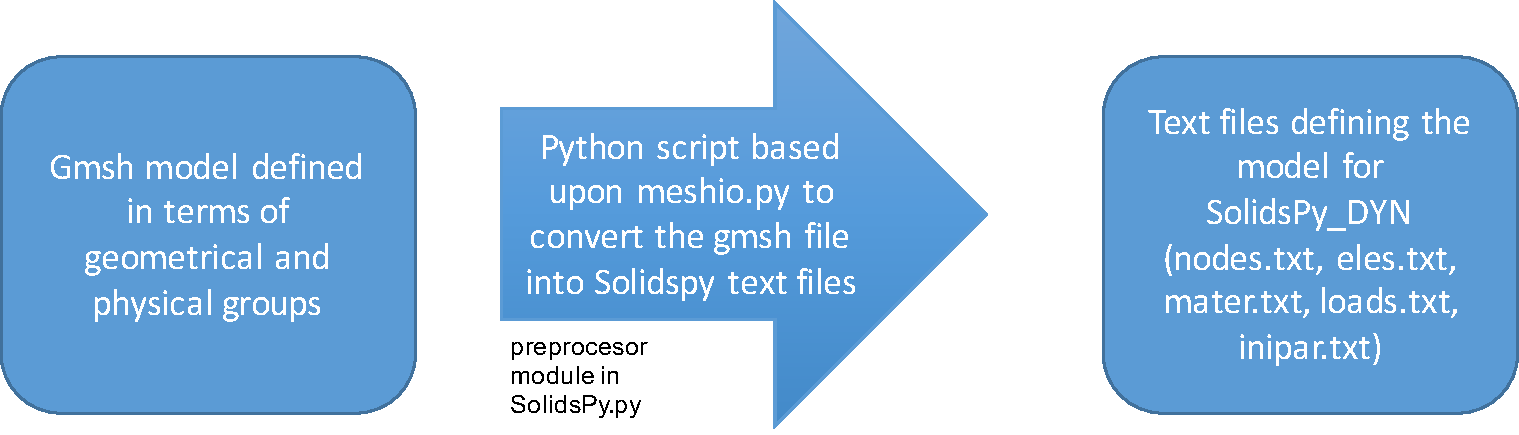
\includegraphics[width=10 cm]{img/modeling.pdf}
  \caption{Creation of a SolidsPy model. The geometry is built and discretized with Gmsh and SolidsPy text files are later written out by meshio.py.}
  \label{fig:modeling}
\end{figure}

In what follows we make a description of each one of the 5 {\bf SolidsPy\_DYN} text files. 

\subsection{Elements data}
Each {\bf SolidsPy\_DYN} finite element model requires a text file (eles.txt) with the following information for each element in the mesh:
\inputminted[mathescape,
               numbersep=5pt,
               gobble=0,
               frame=lines,
               framesep=2mm]{c}{elesT.txt}
               
where

\begin{itemize}
\item {\bf ele\_id}: Integer defining the id for the current element. The elements in the text file must be listed in consecutive ascending order.
\item {\bf ele\_tag}: Integer defining the type of element according to (1): 4-noded bi-lineal element, (2): 6-noded quadratic triangle, (3): 3-noded linear triangle.
\item {\bf mat\_tag }: An integer number defining the material profile associated to the current element. A material profile is a st of material parameters defining the elastic properties of a given material. These are defined in the mater.txt file.
\item{\bf  n1  n2  ...nN}: For a N-noded element a list of N nodal numbers defining the nodes of the current element.
\end{itemize}

The eles.txt file can be created out of a Gmsh file by the python subroutine {\bf ele\_writer()} available in the {\bf preprocesor} module of the program.

\subsection{Nodal data}
Each {\bf SolidsPy\_DYN} finite element model requires a text file (nodes.txt) with the following information for each nodal point in the mesh

\inputminted[mathescape,
               numbersep=5pt,
               gobble=0,
               frame=lines,
               framesep=2mm]{c}{nodesT.txt}

where
\begin{itemize}
\item {\bf id}: Integer defining the id for the current node. The nodes in the text file must be listed in consecutive ascending order.
\item {\bf x-coord}: Horizontal coordinate of the nodal point in a cartesian reference system.
\item {\bf y-coord}: Vertical coordinate of the nodal point in a cartesian reference system.
\item{\bf  BC-x}: Horizontal displacement boundary condition flag at the current node. A value of -1 implies that the degree of freedom is restrained and a value of 0 that it is free.
\item{\bf  BC-y}: Vertical displacement boundary condition flag at the current node. A value of -1 implies that the degree of freedom is restrained and a value of 0 that it is free.
\end{itemize}

The nodes.txt file can be created out of a Gmsh file by the python subroutine {\bf node\_writer()} available in the {\bf preprocesor} module of the program. Since the displacement boundary conditions are different than 0 only at a limited set of nodes these can be written using the python subroutine {\bf boundary\_conditions()} available in the {\bf preprocesor} module of the program.
               

\subsection{Materials data}
Each {\bf SolidsPy\_DYN} finite element model requires a text file (mater.txt) with the following information for each material profile in the mesh. A material profile is a set of parameters corresponding to a given material. Each material profile is defined by a line of text with the following parameters:

\inputminted[mathescape,
               numbersep=5pt,
               gobble=0,
               frame=lines,
               framesep=2mm]{c}{materT.txt}

where
\begin{itemize}
\item $E$      : Young modulus
\item $\nu$   : Poisson's ratio.
\item $\rho$  : Mass density.
\item $D_1$  : Constant for mass proportional damping.
\item $D_2$  :Constant for stiffness proportional damping.
\end{itemize}

The mater.txt file must be manually created by the user.

\subsection{Loading data}
Each {\bf SolidsPy\_DYN} finite element model requires a text file (loads.txt) with the following information for each loaded node in the mesh.
\inputminted[mathescape,
               numbersep=5pt,
               gobble=0,
               frame=lines,
               framesep=2mm]{c}{loadsT.txt}
               
where

\begin{itemize}

\item {\bf Node}: Node number for the current load.
\item {\bf $F_x$}: Magnitude of the nodal point load in the horizontal direction.
\item {\bf $F_y$}: Magnitude of the nodal point load in the vertical direction.

\end{itemize}

{\bf SolidsPy\_DYN} only considers nodal point loads, and thus surface tractions must be converted into nodal point loads. This conversion can be made using the Gmsh file and the python subroutine {\bf loading()} available in the {\bf preprocesor} module of the program.


\subsubsection{Time dependence of the loading data}

All the loads in {\bf Solidspy\_DYN} are specified with a time variation in terms of a Ricker pulse. This time function is defined as follows:
 
 \[A = \left( {1 - 2{\pi ^2}f_c^2{t^2}} \right){e^{ - {\pi ^2}f_c^2{t^2}}}\]
 
 where $f_c$ is the central frequency. In {\bf Solidspy\_DYN} the pulse is centered as specified by $t_c$.
 
 
 \begin{figure}[H]
  \centering
  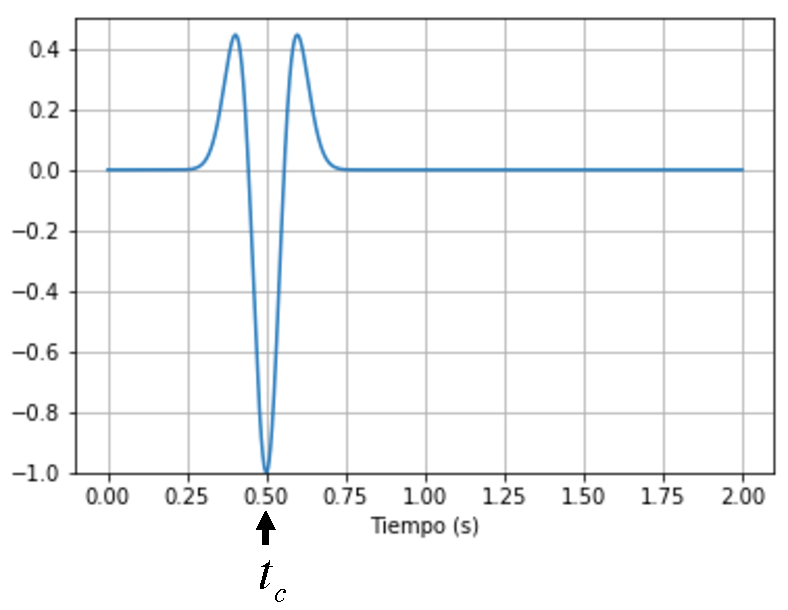
\includegraphics[width=6 cm]{img/pulse.pdf}
  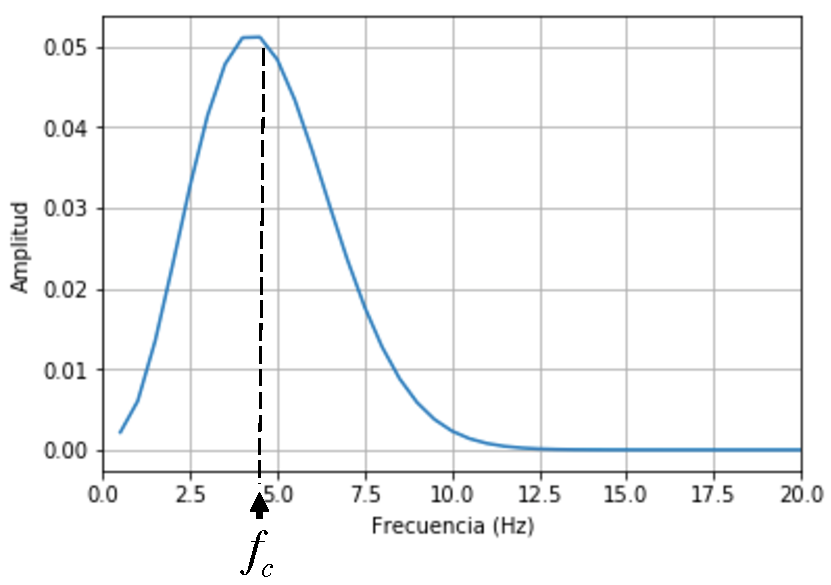
\includegraphics[width=6 cm]{img/fourier.pdf}
    \caption{Time function and Fourier spectra for the Ricker pulse. The signal is characterized by its central time $t_c$ and its dominant frequency parameter $f_c$}
  \label{fig:mesh}
\end{figure}

The load is defined using data combined in two files. In the loads.txt file the user must specify a list of nodes with the amplitude of the load along each degree of freedom. The remaining parameters corresponding to the time variation of the load and completely defining the Ricker pulse are indicated in the integration parameters file of the model as described next.


\subsection{Time dependent data}
Each {\bf SolidsPy\_DYN} finite element model requires a text file (inipar.txt) with the following time dependent information for the analysis:

\inputminted[mathescape,
               numbersep=5pt,
               gobble=0,
               frame=lines,
               framesep=2mm]{c}{iniparT.txt}
               
where

\begin{itemize}
\item {\bf $dt$}   : Time step for the incremental analysis.
\item {\bf $T$}    : Duration of the analysis.
\item {\bf $t_c$} : Central time in the Ricker pulse.
\item {\bf $f_c$} : Central frequency in the Ricker pulse.
\end{itemize}


\section{Definition of a finite element model for SolidsPy\_DYN using Gmsh}

This section describes the basic components and steps for the construction of a finite element model to conduct dynamic analysis with {\bf Solidspy\_DYN}. It is assumed that the user is familiar with Gmsh. There are several tutorials in the TUTORIALS folder of the code. 

The model construction process is explained with reference to the problem shown in \cref{fig:placa}  corresponds to a rectangular plate composed of two different materials  and submitted to a point load with time variation defined by a Ricker pulse applied at the top.

\begin{figure}[h]
  \centering
  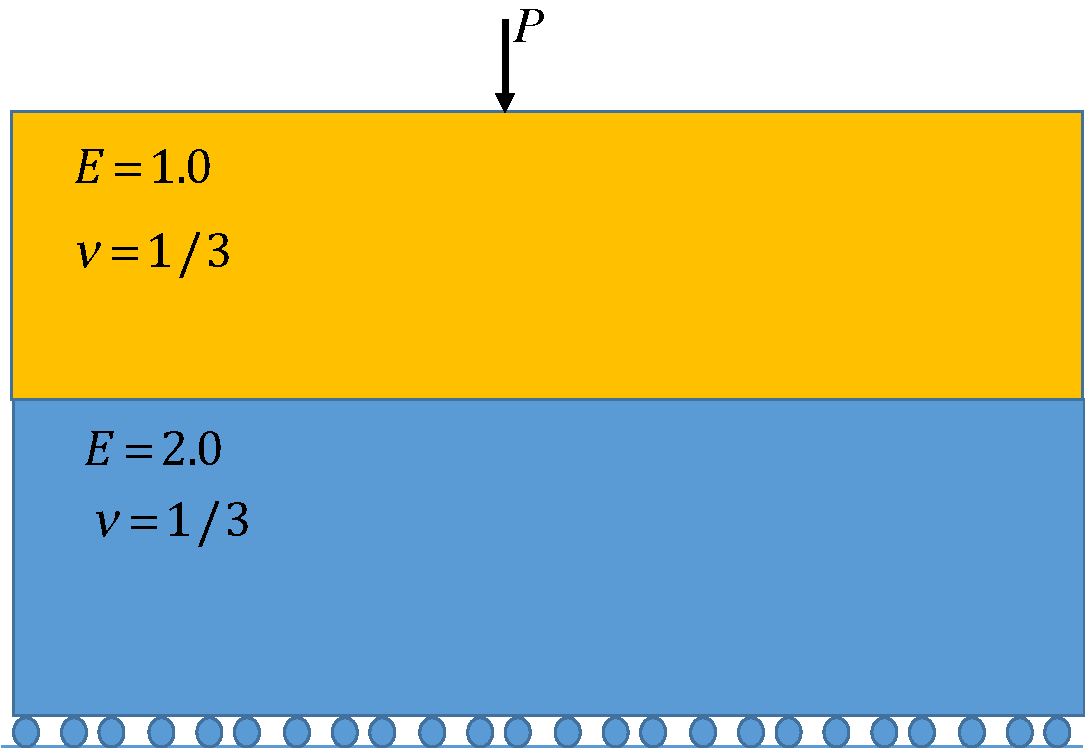
\includegraphics[width=8 cm]{img/placa.pdf}
  \caption{Rectangular plate conformed by two different materials under a time varying point load at the free surface.}
  \label{fig:placa}
\end{figure}

The construction of a model in {\bf Gmsh} involves the generation of geometrical elements defining all the points, lines and planes required to build the geometry and physical groups corresponding to special sets of points, lines and planes (or surfaces) where particular modeling conditions are expected to occur. The names or labels assigned to the physical groups are later associated to the specific elements of the mesh pertaining to these groups.

For instance if nodal points are to be applied over a given line of the model, it is convenient to define that specific line as physical line. Later during the mesh creation process all the nodes lying along that specific physical line will be stored in an independent data structure facilitating the modeling process. The following sections describe the generation of the geometrical and physical groups required in a {\bf Gmsh} model for {\bf SolidsPy\_DYN}\footnote{The following link contains a series of videos showing the modeling process for this example \url{<https://www.youtube.com/channel/UCNhX9Z5wkEk_JhlSuIo8A4Q>}}.

\subsection{Geometrical entities}
The geometrical entities of the model are shown in \cref{fig:geometrical} together with the conventions used to describe each entity. The corresponding entities or groups are in hierarchical order points, lines (formed by points), line loops (formed by groups of lines generating a closed figure) and plane surfaces (formed by a line loop). The current model contains two plane surfaces since we will be using two different materials in each part of the domain. When creating the model it is convenient to use parameters for all the dimensions as this will facilitate the execution of several analysis later. Here we will assume that the model is of width $L$, while the lateral faces are specified by dimensions $H1$ and $H2$. As additional parameter we will use the characteristic element size $hc$ to be specified as a fraction of the total width.

\begin{figure}[h]
  \centering
  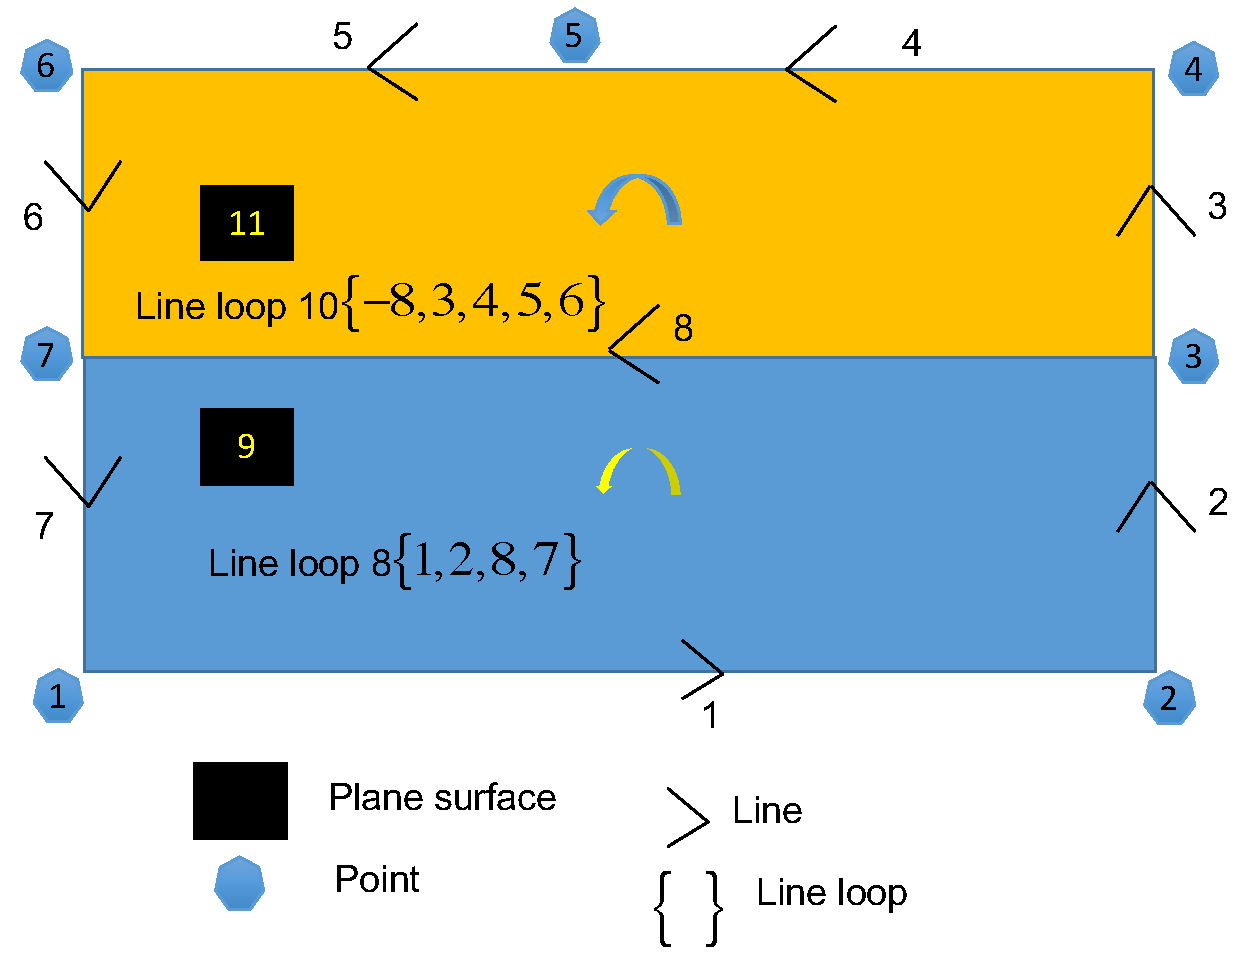
\includegraphics[width=8 cm]{img/geometrical.pdf}
  \caption{Geometrical entities for the model.}
  \label{fig:geometrical}
\end{figure}

\subsection{Physical entities}
The physical groups in the model are described in \cref{fig:physical}. These correspond to the two physical surfaces labeled (100) and (200) respectively; a physical line, labeled (400) and a physical point with the label (500). These names will be assigned to all the nodes and elements that coincide with those specific groups. The physical surfaces are required in order to indicate which elements are assigned each material profile. The physical line is required in order to identify the nodes at which displacement boundary conditions are to be imposed and the physical node is required in order to specify the loading node. Each physical group is described next:

\begin{itemize}
\item Physical surface $100$: Top material layer.
\item Physical surface $200$: Bottom material layer.
\item Physical line $400$: Bottom surface with all restrained vertical and horizontal displacements.
\item Physical point $500$: Localization of the dynamic point load.
\end{itemize}

\begin{figure}[h]
  \centering
  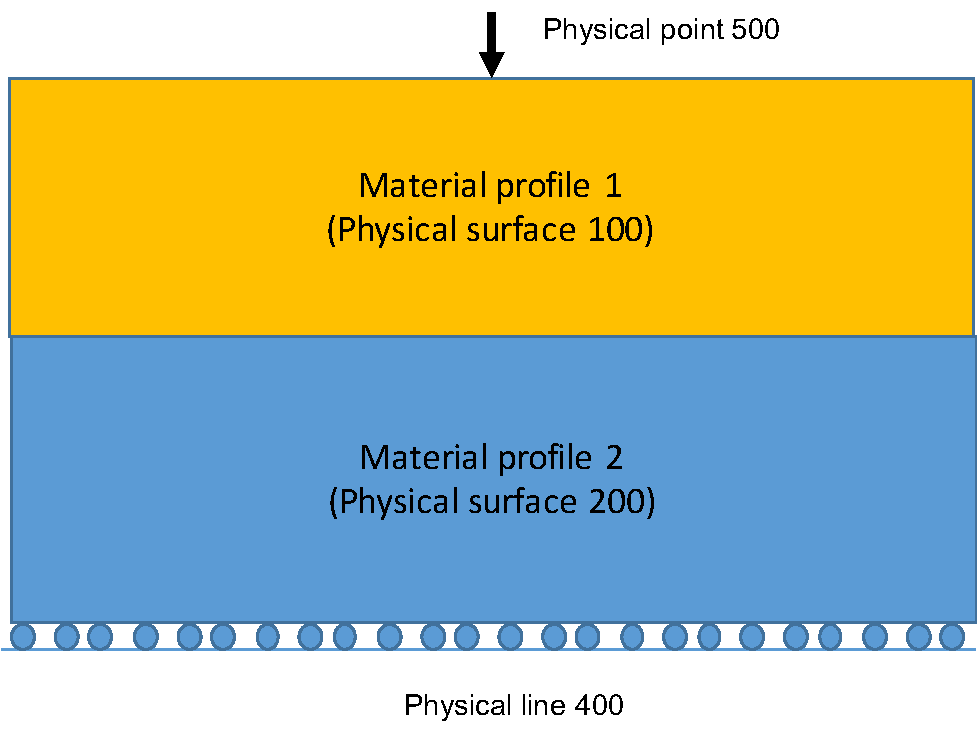
\includegraphics[width=8 cm]{img/physical.pdf}
  \caption{Physical entities for the model.}
  \label{fig:physical}
\end{figure}

The model defined in terms of geometrical and physical groups is returned by {\Gmsh} as a file with extension \texttt{.geo}. The specific \texttt{.geo} file for the example problem is shown next.

\inputminted[mathescape,
               numbersep=5pt,
               gobble=0,
               frame=lines,
               framesep=2mm]{c}{bimaterial.geo}
               
After conducting a couple of mesh refinements the discretized model should look as shown in \cref{fig:mesh}

\begin{figure}[H]
  \centering
  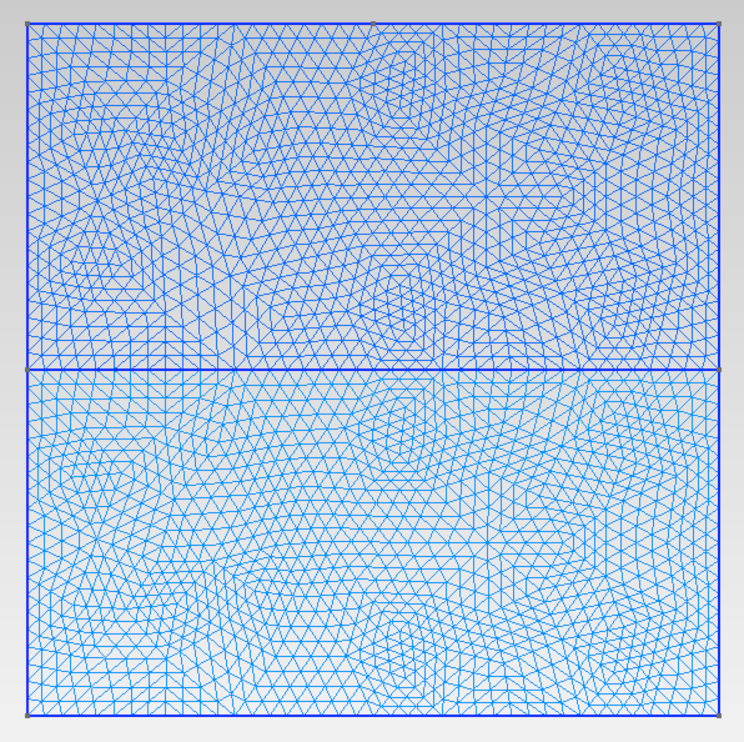
\includegraphics[width=8 cm]{img/mesh.pdf}
  \caption{Finite element mesh conformed of linear triangular elements.}
  \label{fig:mesh}
\end{figure} 



\section{Generation of text files from the Gmsh model}
\label{meshio}
The input data in terms of text files for the finite element code must now be defined using the {\bf gmsh} model. This is achieved using subroutines available in the {\bf preprocessor} module of {\bf SolidsPy}. These routines are written on top of the input-output python based module {\bf meshio}. These subroutines are essentially required to write the nodes.txt and elements.txt files required by {\bf Solidspy\_DYN} which may result massive and cumbersome to process. The python script that produces the input files for the current example is described next.


\inputminted[mathescape,
               numbersep=5pt,
               gobble=0,
               frame=lines,
               framesep=2mm]{c}{bimaterial.py}


In the first block we import the required modules for the script. In particular the script requires the module {\bf meshio} and the module {\bf preprocesor} from {\bf solidspy}.

After the modules have been imported, the first line of code uses {\bf meshio} to read the {\bf gmsh} mesh. In this case the mesh has been saved with the name {\bf bimaterial.msh}. Once the mesh is read all the model is stored in python dictionaries ready to be processed. The process of manipulating the dictionaries and extracting the data for the text files is done with subroutines available in the module  {\bf preprocesor} from {\bf solidspy} and this implies that for these routines to be available {\bf solidspy} has been previously installed.

In the first part the points and point\_data dictionaries are used by the subroutine node\_writer to write an array with the nodal point data in the format required by the finite element code.

The element processing is performed by the element writer subroutine. This subroutine must be invoked as many times as there are physical surfaces in the model. The subroutine uses the following input parameters:

\begin{itemize}
\item  The python dictionaries cells and cell\_data storing all the element information.
\item  The name for the element used in the current surface according to {\bf gmsh} which in this case corresponds to "triangle" for the lineal triangles.
\item The number of the surface being processed according to {\bf gmsh}. In this case we have defined physical surfaces with numbers $100$ and $200$ for the top and bottom surface respectively.
\item A number identifying the type of element according to {\bf Solidspy\_DYN} which in this case is $3$ since we are using a triangular lineal element.
\item  A number identifying the material profile to be used in the current surface. In this case the top surface has been assigned the material properties defined in the material profile $0$ while the bottom surface has been assigned those from material profile $1$.
\item An integer parameter specifying where the current surface should start counting elements. In this particular problem the element writer starts counting elements from $0$ in the first surface and from {\bf nini} in the second surface where {\bf nini} is the last element from the previous surface.
\end{itemize}

Upon execution this subroutine returns an array with the elemental information for the current surface but now written in {\bf Solidspy\_DYN} format and an integer number indicating the total number of elements contained in that surface. This number is required if processing several surfaces since this marks down where the next element counting should begin.

The next part of the script specifies the boundary conditions. Thus boundary conditions subroutine requires the following input parameters:

\begin{itemize}
\item The python dictionaries cells and cell\_data storing all the element information.
\item An integer specifying the name assigned to the line where the current boundary condition is to be imposed. In this case we have used the number $400$ to specify the bottom line of the model.
\item The array containing the nodal data and generated by the nodes writer subroutine. This array will be modified by the boundary conditions subroutine.
\item Two boundary condition specifiers indicating if the horizontal and vertical degrees of freedom are free (value $=0$) or restrained (value $=-1$).
\end{itemize}

The final part of the script uses the previously generated arrays and writes the corresponding text files. Since we have processed two physical surfaces the two resulting arrays must be concatenated into a single element array ready for output. This is done using the python function append.

\section{Visualization of displacement time histories}
\subsection*{Animated view of the propagation patterns}
In wave propagation analysis it is common to develop conceptual understanding of a given solution based upon the propagation pattern experienced by the propagated wave field. In {\bf Solidspy\_DYN} these visualizations can be realized  using the external open-free visualization software {\bf Paraview}. By default {\bf Solidspy\_DYN} writes ready-to-process VTK files that can be read by {\bf Paraview}. Each output VTK file corresponds to a snapshot of the solution at given time instant.  These files are stored by {\bf Solidspy\_DYN} in the folder /MESHES/VTKs.

\subsection*{View of the surface displacements at a line of points}
A second possibility for the visualization of results is to simultaneously plot the time response for a series of points located along a given line. If the resulting time signals are plotted with the amplitudes progressively scaled by a constant factor the plot gives a physical sense of the propagation pattern.

The generation of results for this type of visualization requires the creation of an additional file, {\bf salida.txt}, storing the identification numbers for the set of response points. This file is created directly from the same script that generates the text files for the model after adding the function {\bf respuesta ()}. This function extracts the nodal identifiers located along a previously defined physical line and writes the required text file.

The second step required to obtain the sheet-like visualization of the response is to execute the analysis within a particular script. The script executes the following steps:

\begin{itemize}
\item Executes the code and computes the time history of displacements at all the nodes. This solution is stored in the array {\bf U}.
\item Loads the text file {\bf salida.txt} into the array {\bf salida}.
\item Invokes the post-processing function {\bf sheets} using as input parameters the array {\bf salida} and the solution array {\bf U}. This function writes down the response into a second file named {\bf respuesta.txt}.
\item Load the file {\bf respuesta.txt} into the array {\bf vals}.
\item Use either of/or both functions {\bf plot_sheet} and {\bf plot_pcolor} using as input parameter the array {\bf vals} to plot the solution.
\end{itemize}

An example of the sheet-like visualization of the results is shown in \cref{fig:sabanas}, while the specific function {\bf respuesta ()} that generates the file for output and the script for execution of the code in post-processing mode are included at the end.

\begin{figure}[H]
  \centering
  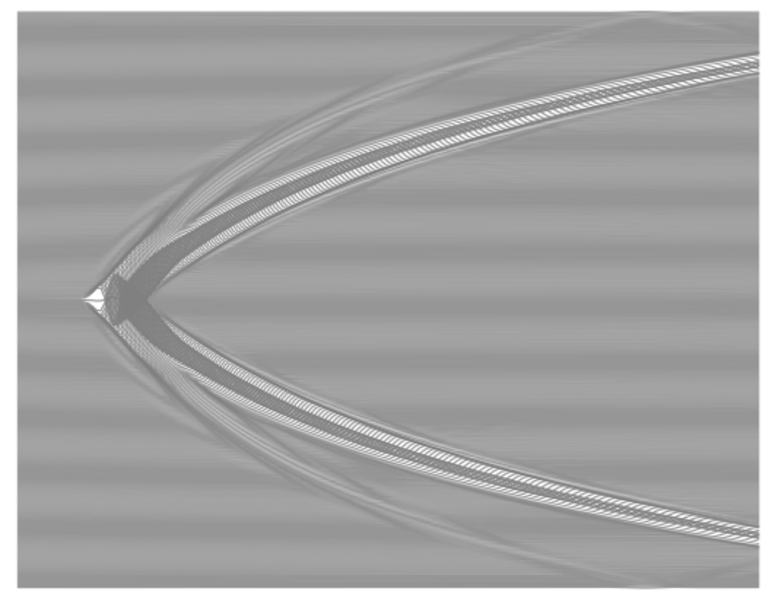
\includegraphics[width=8 cm]{img/sabana1.pdf}\\
    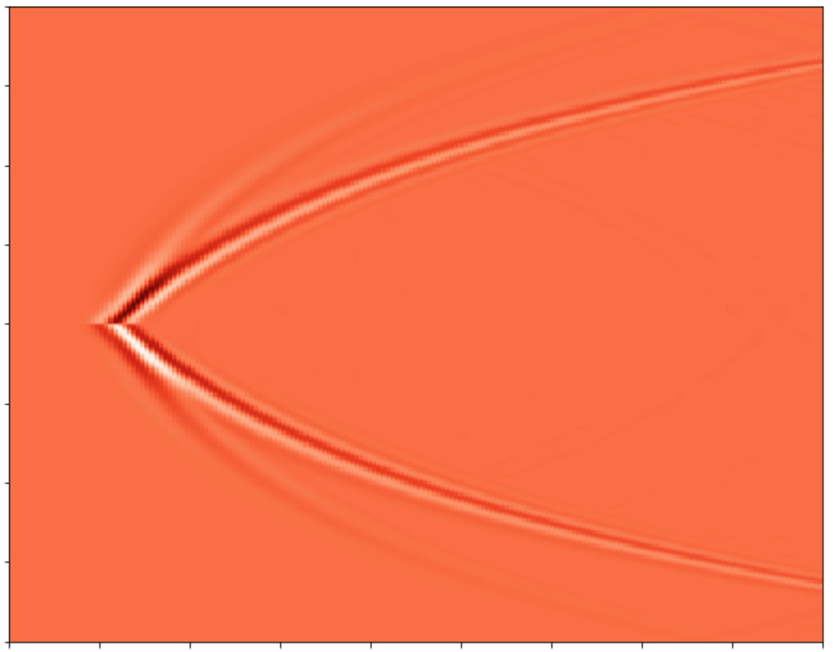
\includegraphics[width=8 cm]{img/sabana2.pdf}
  \caption{Visualization of response time histories at a set of nodal points located along the same line.}
  \label{fig:sabanas}
\end{figure} 



\inputminted[mathescape,
               numbersep=5pt,
               gobble=0,
               frame=lines,
               framesep=2mm]{c}{generador.py}
               
\inputminted[mathescape,
               numbersep=5pt,
               gobble=0,
               frame=lines,
               framesep=2mm]{c}{ejecucion_postpr.py}


               

\bibliographystyle{gji}
\bibliography{bibliografia}



      

             


\end{document}